\documentclass[a4paper,12pt]{report}

\usepackage[T1]{fontenc} % font encodings
\usepackage[utf8]{inputenc} % use utf8 as encoding
\usepackage{lmodern} % use Latin Moderna
\usepackage[french]{babel} % set french as language
\usepackage{graphicx} % manipulate image
\usepackage{hyperref} % use hyper reference
\usepackage[newfloat]{minted} % syntax highlighting
\usepackage{caption} % for, well, caption
\usepackage[use-files]{xsim} % exercise helper
\usepackage{titlesec} % manipulate title
\usepackage{xr} % cross-document reference
\usepackage{xcolor} % manipulate color
\usepackage{enumitem} % better list
\usepackage{tikz} % for graphics
\usepackage{float} % for figure position
\usepackage{appendix} % for appendix
\usepackage{stmaryrd} % for maths things

\externaldocument[appendix-]{./content/appendix}

% load some tikz library
\usetikzlibrary{positioning}
\usetikzlibrary{shapes.geometric, arrows}

% define code block background color
\definecolor{bg}{rgb}{0.95,0.95,0.95}
\setminted[java]{breaklines,linenos,autogobble,bgcolor=bg}
\setminted[xml]{breaklines,linenos,autogobble,bgcolor=bg}
\setmintedinline[java]{bgcolor={}} 

% remove useless formating of chapter
\titleformat{\chapter}
  {\normalfont\LARGE\bfseries}{\thechapter}{1em}{}
\titlespacing*{\chapter}{0pt}{3.5ex plus 1ex minus .2ex}{2.3ex plus .2ex}

% define a macro for our code-style word
\newcommand{\code}[1]{%
    \texttt{#1}%
}

% add all the exercices to the TOC
\newcommand\addsubsec[1]{%
  \section*{#1}%
  \addcontentsline{toc}{section}{\numberline{\GetExerciseProperty{counter}} \GetExerciseProperty{subtitle}}%
}

% custom exercise environment
\DeclareExerciseEnvironmentTemplate {custom}
  {
    \GetExerciseHeadingF { \subsection* }
    {
      \XSIMmixedcase { \GetExerciseName } \nobreakspace
      \GetExerciseProperty {counter}
      \IfInsideSolutionF
        {
          \IfExercisePropertySetT {subtitle}
            { { \normalfont \GetExerciseProperty {subtitle} } }
        }
    }
  }
  { \par }

\xsimsetup{
  exercise/the-counter = \arabic{section}.\arabic{exercise}, % for "Exercice <section>.<number>
  exercise/heading=\addsubsec,
  exercise/template=custom
}

% some tikz styles
\tikzset{
    start/.style={draw, rectangle, rounded corners, minimum height=1cm, minimum width=4cm, fill=gray!50},
    class/.style={draw, rectangle, rounded corners, minimum height=1cm, minimum width=4cm},
    arrow/.style={very thick,->,>=stealth}
}

\begin{document}
\begin{titlepage}

{\centering

\includegraphics[width=0.15\textwidth]{./media/murphy.png}\\

\vspace{1cm}

{\scshape\LARGE ESIEE Paris \\}

\vspace{2.5cm}

{\huge\bfseries Rapport projet Zuul\\}

\vspace{2cm}

{\Large Corentin POUPRY\\}

\vfill

supervisé par\\
Denis Bureau

\vfill
	
{\large 2020 - 2021\\}
}


\end{titlepage}

\tableofcontents

\setlength{\parskip}{1em}

\chapter{Présentation}

\section{Auteur}

\noindent
Corentin POUPRY, étudiant à l'ESIEE Paris en E1, promotion 2025.

\section{Thème}

\noindent
Murphy Law, un détective, doit faire la lumière sur l'enquête confiée.

\section{Résumé du scénario}

Vous vous attendiez à tomber sur un super jeu de science-fiction proposé par un étudiant talentueux. Cependant, la réalité est tout autre et vous vous retrouvez au bureau d'un curieux détective. Ce détective, bien décidé à vous aider à faire la lumière sur votre cas atypique, c'est Murphy Law, et c'est lui qu'on appelle quand tout va mal.

\section{Scénario détaillé}

Le Joueur (notons la majuscule) est un personnage à part entière de l'histoire, bien que l'utilisateur joue au travers de Murphy Law. Le Joueur apparaît au début de la narration complètement perdu et à la recherche du jeu de science-fiction promis par le talentueux étudiant dans son rapport. Murphy Law, détective, se demande par quel moyen Le Joueur a pu arriver dans son agence alors que, manifestement, il ne fait même pas partie du schéma narratif du jeu. Quelque chose cloche, quelque chose ne tourne pas rond.\\

Murphy Law décide de partir mener l'enquête en allant voir une source pouvant l'aider dans cette enquête. Avec Le Joueur, il monte dans sa voiture (voir \hyperlink{section.1.6}{Plan}), cependant, la structure du jeu commence à se corrompre, à changer dangereusement sans raison, provoquant la stupéfaction chez les deux protagonistes. Murphy accélère pour semer les incohérences de narration. Alors qu'ils roulent vers leur contact à toute allure, Murphy commence à perdre le contrôle de la situation jusqu'à qu'un arbre apparaisse devant la voiture provoquant un accident.\\

Murphy Law et Le Joueur se réveille dans un grand escalier avec des dorures et un dôme imposant surmontant la pièce. Après l'irruption d'un majordome disant qu'on les cherche partout, Murphy et Le Joueur réalisent qu'ils passé dans l'univers d'un autre jeu de la promotion, prenant place à Buckingham Palace. Très vite, Murphy Law et Le Joueur sont accostés par les employés du palais qui les accompagnent dans la salle de réception où il découvre le crise nationale qui frappe le palais: un corgi royal est manquant.

\verb|TODO: pas encore totalement fini|.

Après avoir perdu le joueur et flairant que quelque chose se trame dans son dos, Murphy Law décide alors de se rendre là où tout a commencé : dans la salle de l'ESIEE où Le Joueur avait lancé le jeu. S'en suit une confrontation avec Le Compilateur, qui essayait de manipuler le jeu à sa guise pour que  l'étudiant n'obtienne pas une note à la haute de sont travail. Murphy ressort gagnant de cette confrontation, ce qui lance le dialogue de fin de Planet Wars.\\

\section{Commandes}

\begin{description}[leftmargin=!,labelwidth=\widthof{\bfseries inspect \textit{objet}}]
  \item [go \textit{direction}] Déplace le personnage vers une certaines pièce.
  \item [look] Affiche la position actuelle ainsi que la description de la pièce.
  \item [inspect \textit{objet}] Permet d'inspecter un objet présent dans la pièce.
  \item [help] Affiche un bref résumé ainsi que la position actuelle.
  \item [quit] Quitte le jeu.
\end{description}

\section{Plan}

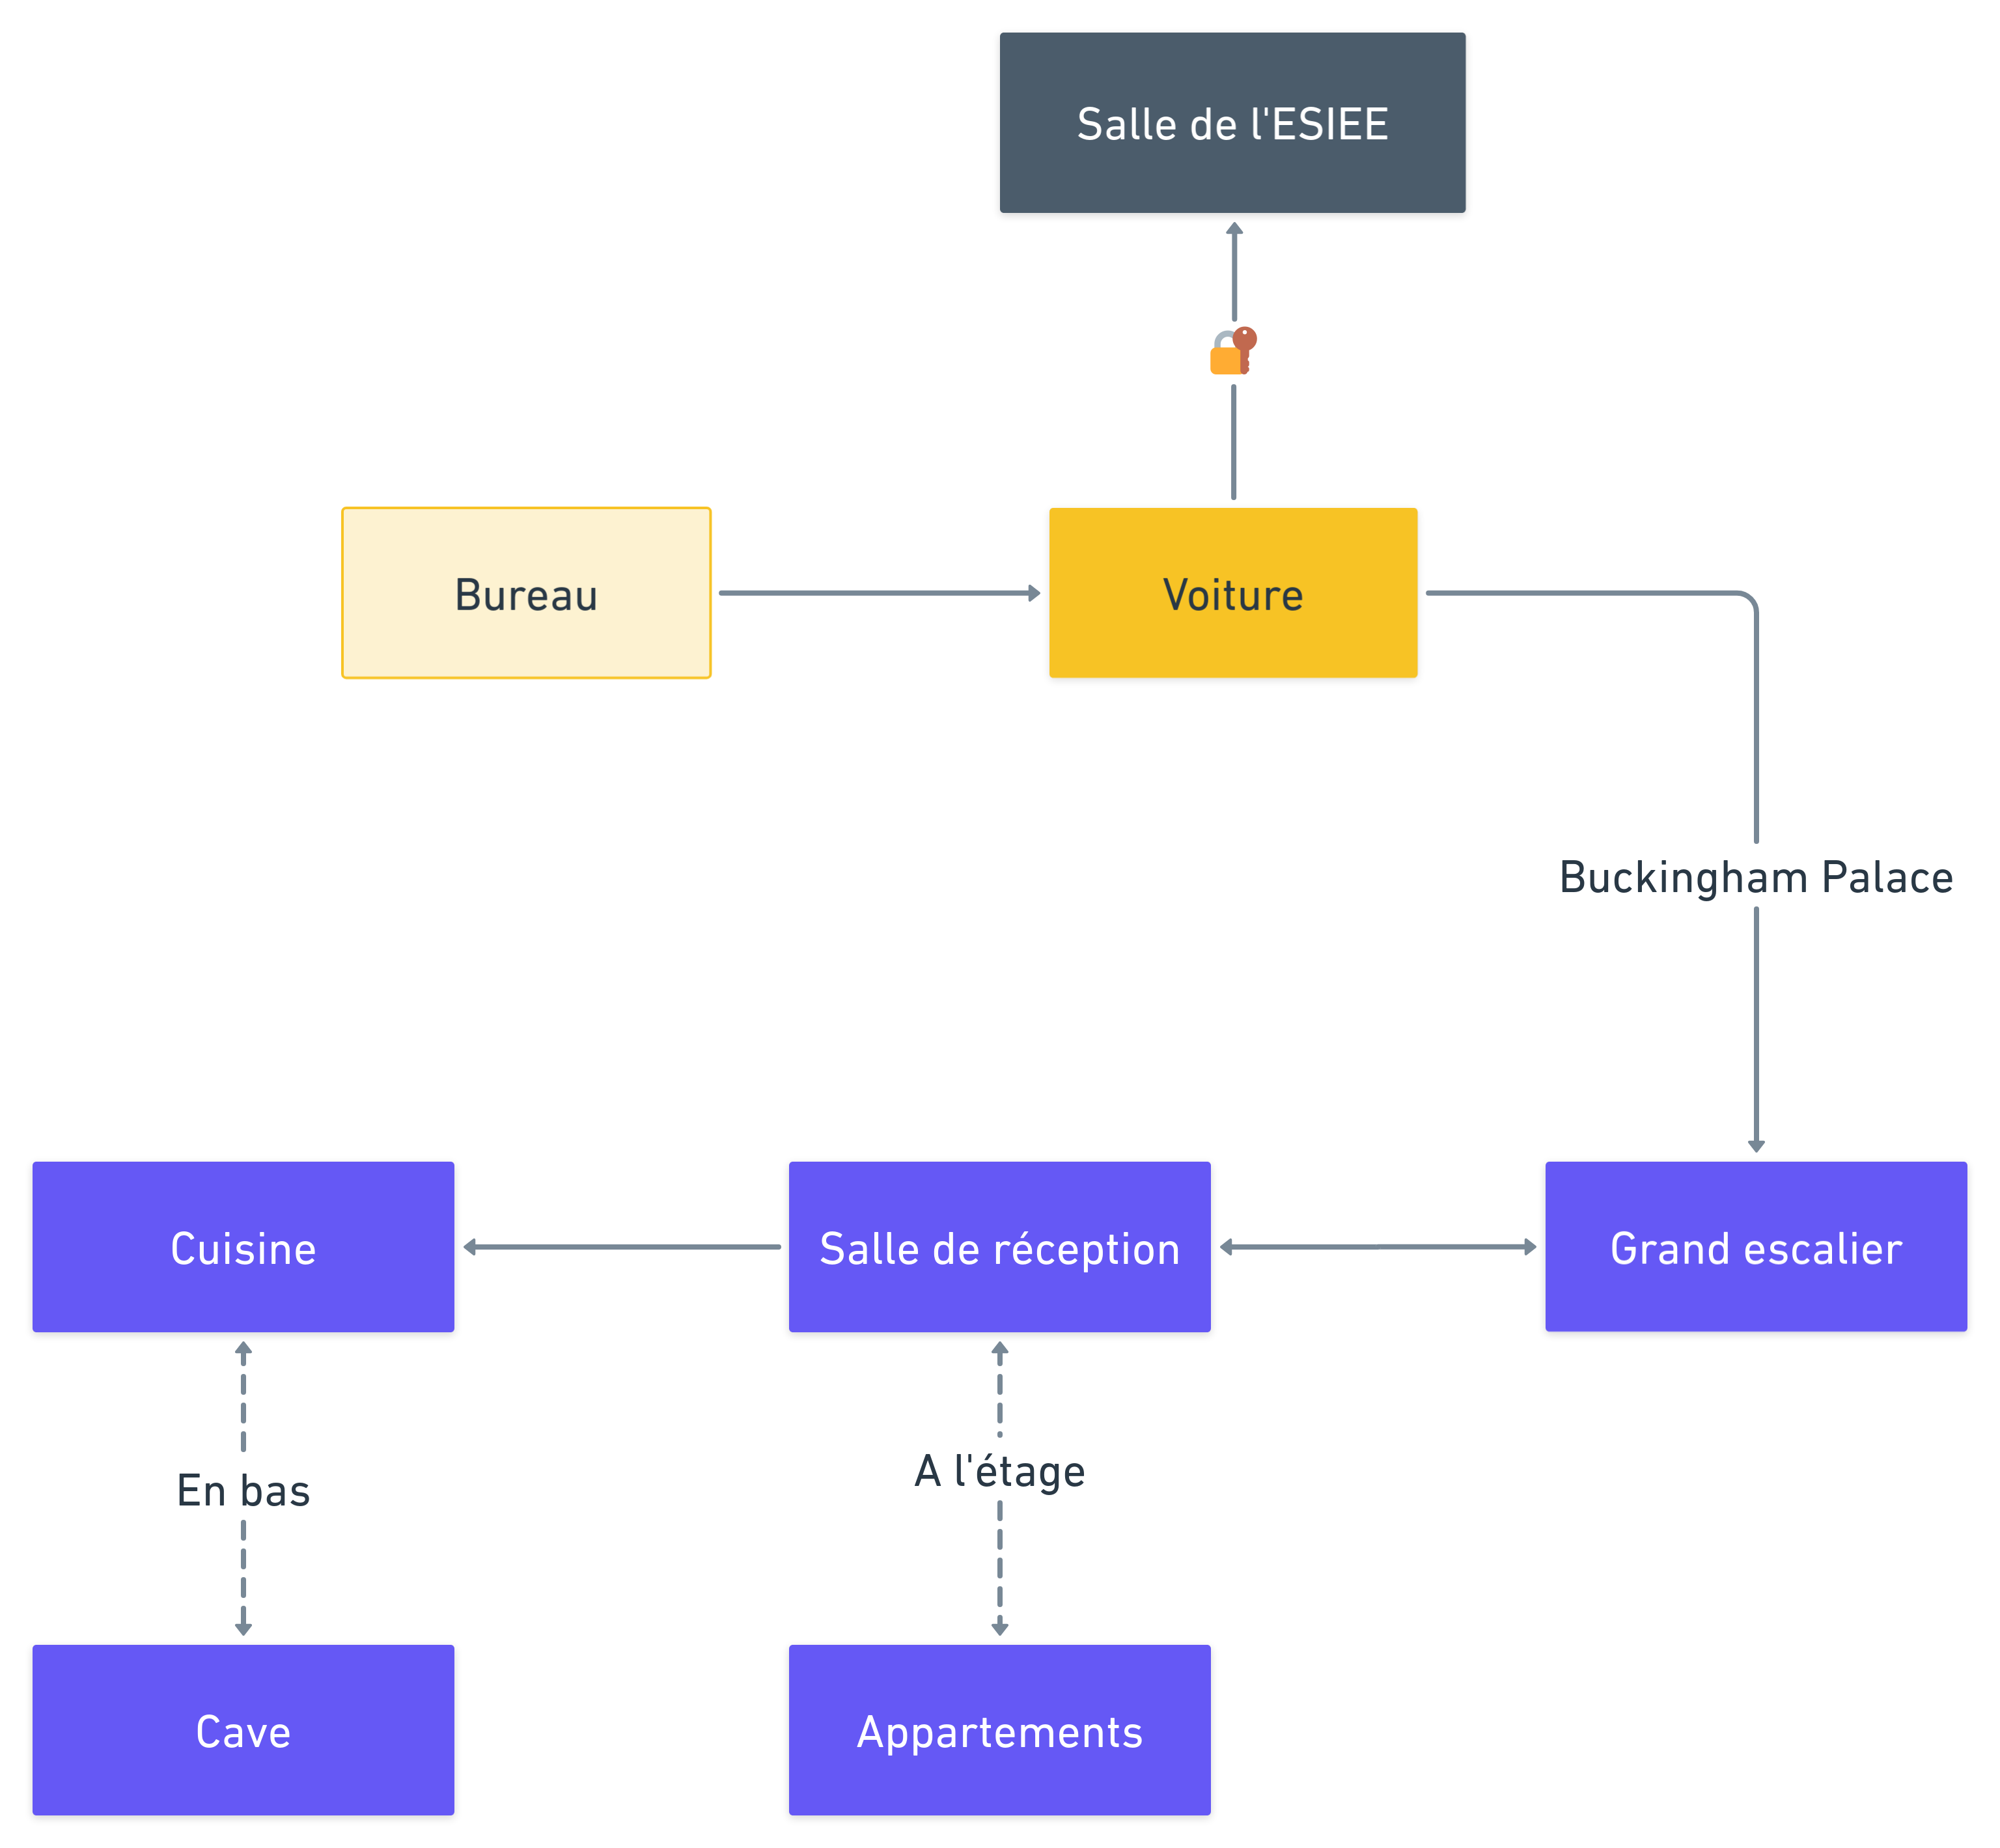
\includegraphics[width=\textwidth,height=\textheight,keepaspectratio]{./media/map.png}\\

\section{Détail des lieux, items, personnages}

\subsection{Lieux}

Seuls les lieux importants à l'avancement et à l'histoire du jeu sont listés ci-dessous.

\begin{description}[leftmargin=!,labelwidth=\widthof{\bfseries Bureau de Murphy}]
  \item [Bureau de Murphy] C'est le lieu où vous commencez votre aventure.
  \item [Voiture] La voiture vous permet de rejoindre certains lieux.
  \item [Grand escalier] C'est l'endroit où vous arrivez à Buckingham Palace.
  \item [Salle de réception] Là où la crise du corgi royal sera expliquée.
  \item [Salle de l'ESIEE] C'est dans cette salle de l'ESIEE que vous avez lancé ce jeu.
\end{description}

\subsection{Personnages}

De la même façon, cette liste ne comprend que les personnages essentiels au scénario. Certains personnages non-joueurs ne sont pas listés ici.

\begin{description}[leftmargin=!,labelwidth=\widthof{\bfseries Le Compilateur}]
  \item [Murphy Law] Le détective et aussi le personnage que vous incarnez. Son rôle est de mener l'enquête pour comprendre par quelles circonstances Le Joueur s'est retrouvé ici.
  \item [Le Narrateur] La voix que vous entendez quand vous jouez. Le Narrateur permet de décrire les scènes \& situations sans sortir de la narration. 
  \item [Le Joueur] C'est vous ! Cependant, Le Joueur est paradoxalement un personnage non jouable qui vous représente tout au long de  l'histoire dans le cadre de la méta-narration.
  \item [Le Compilateur] Le compilateur Java est le grand méchant de l'histoire. Son rôle, manipuler la structure du jeu pour que l'étudiant n'ait pas une note à la hauteur de son travail.
\end{description}

\section{Situations gagnantes et perdantes}

Le Joueur et Murphy Law seront confrontés à des situations de crises où des choix et décisions devront être prises, certains pourront entraîner la mort ou l'immobilisation des protagonistes et donc faire gagner Le Compilateur.\\
La liste des situations perdantes est la suivante :

\begin{description}[align=left,leftmargin=!,labelwidth=\widthof{\bfseries A Buckingham Palace}]
  \item [A Buckingham Palace] \begin{itemize}
    \item Vous ne retrouvez pas le corgi royal.
    \item Vous essayez de fouiller la Reine d'Angleterre.
  \end{itemize}
\end{description}

\section{Commentaires}

Murphy Law est une création originale de \href{http://scp-wiki.wikidot.com/murphy-law-hub}{la Fondation SCP}. Le personnage, les œuvres associées et ce jeu sont tous proposés sous licence \emph{Creative Commons Attribution-ShareAlike 3.0}
 


\chapter{Exercices}

% The first really interesting exercise to write is 7.5. 
% We initialize our counters to match this situation.
\setcounter{section}{7}
\setcounter{exercise}{4}

\begin{exercise}[subtitle=printLocationInfo]

En ré-usinant le code de l'affichage de la localisation et des sorties en une fonction, on s'assure de ne pas répéter cette partie à plusieurs endroits.

\begin{minted}{java}
private void printLocationInfo() {
    Room vCurrent = this.aCurrentRoom;
    System.out.printf("You are %s%n", vCurrent.getDescription());
   
    System.out.print("Exits: ");
    if (vCurrent.aEastExit != null) System.out.print("east ");
    if (vCurrent.aNorthExit != null) System.out.print("north ");
    if (vCurrent.aSouthExit != null) System.out.print("south ");
    if (vCurrent.aWestExit != null) System.out.print("west ");
    System.out.println();
}
\end{minted}
\end{exercise}

\begin{exercise}[subtitle=getExit]

Dans cet exercice, on se rend compte que le système "un attribut = une sortie" n'est pas le plus optimal (imaginons un hub ayant une dizaines de sorties par exemple, ce qui deviendrait problématique pour la lisibilité et la maintenance du code). L'idée étant de limiter le couplage entre la classe \verb|Room| et les autres classes. Pour cela, on cherchera à limiter la dépendance aux attributs de Room et plutôt passer par une fonction pour récupérer les sorties, ce qui permet de ne gérer la logique des sorties que du côté de \verb|Room|.\\ 

\textbf{Notes:} Notons qu'il reste un problème dans \verb|printLocationInfo| à cause de ce changement, problème abordé dans les exercices qui suivent. On peut aussi émettre une critique quant à la façon de fonctionner de \verb|getExit|: si jamais on passe \verb|"North"| à la place de \verb|"north"| par inadvertance, on aura comme valeur de retour \verb|null|. Une solution serait d'utiliser des \verb|enum|.

\begin{minted}{java}
public Room getExit(final String pDirection) {
    switch (pDirection) {
        case "north":
            return this.aNorthExit;

        case "east":
            return this.aEastExit;

        case "south":
            return this.aSouthExit;

        case "west":
            return this.aWestExit;

        default:
            return null;
    }
}
\end{minted}
\end{exercise}

\begin{exercise}[subtitle=getExitString]
Le dernier changement a impacté la façon dont \verb|printLocationInfo| fonctionne. Pour le résoudre, on écrit une nouvelle méthode \verb|getExitString| et, fort de ce changement, on ré-usine \verb|printLocationInfo|.

\begin{minted}{java}
public String getExitString() {
    String vResult = "Exits: ";

    if (this.aEastExit != null) vResult += "east ";
    if (this.aNorthExit != null) vResult += "north ";
    if (this.aSouthExit != null) vResult += "south ";
    if (this.aWestExit != null) vResult += "west";

    return vResult;
}

private void printLocationInfo() {
    Room vCurrent = this.aCurrentRoom;

    System.out.printf("You are %s%n", vCurrent.getDescription());
    System.out.println(vCurrent.getExitString());
}
\end{minted}
\end{exercise}

\begin{exercise}[subtitle=HashMap et setExit]

Maintenant que le couplage entre \verb|Room| et \verb|Game| est faible, on peut remplacer les détails de l'implémentation sans risquer de casser quelque chose. On utilise une structure de données \verb|HashMap| et on doit changer les méthodes de \verb|Room| en conséquence. On en profite aussi pour remplacer \verb|setExits|, devenue inutile, par \verb|setExit|.

\begin{minted}{java}
public Room setExit(final String pDirection, final Room pExit) {
    this.aExits.put(pDirection, pExit);

    return this;
}

public Room getExit(final String pDirection) {
    return this.aExits.get(pDirection);
}
\end{minted}
\end{exercise}

\textbf{Note :} J'ai ajouté en plus de ce que l'exercice demandait la dernière ligne \mintinline{java}{return this;} pour pouvoir chaîner les appels de \verb|setExit| comme ci-dessous:

\begin{minted}{java}
office.setExit("east", car)
      .setExit("north", kitchen)
      .setExit("west", library);
\end{minted}

\begin{exercise}[subtitle=keySet]

\verb|getExitString| doit elle aussi être modifiée. Plutôt que de tester la présence de certaines valeurs dans la \verb|HashMap| (du type "north", "east", "down", "up"...), on peut énumérer les différentes clés qui composent la \verb|HashMap| des sorties.

\begin{minted}{java}
public String getExitString() {
    String vResult = "Exits : ";
    for (String vExit : this.aExits.keySet())
        vResult += vExit + " ";

    return vResult;
}
\end{minted}
\end{exercise}

\begin{exercise}[subtitle=Fonctionnement de keySet et Javadoc]

Reprenons le code intéressant de l'exercice précédent et intéressons-nous à son fonctionnement.

\begin{minted}{java}
for (String vExit : this.aExits.keySet())
    vResult += vExit + " ";
\end{minted}

Ce code marche car \verb|keySet| renvoit un \verb|Set| qui est énumérable et utilisable par la boucle for-each.\\

La différence entre un \verb|Set| et une liste normale (un tableau) est que le \verb|Set| ne peut pas contenir deux mêmes éléments.\\

Pour la Javadoc, la documentation de \verb|Game| contient beaucoup moins de méthode que \verb|Room| car l'encapsulation fait que seul \verb|play| est publique pour \verb|Game|, tandis que \verb|Room| doit exposer beaucoup plus de méthodes \verb|public| pour être utilisée par \verb|Game|.

\end{exercise}

\begin{exercise}[subtitle=getLongDescription]

Toujours dans la logique de la conception dirigée par responsabilités, on déplace la création de la description dans la classe \verb|Room|.

\begin{minted}{java}
public String getLongDescription() {
    return "Vous êtes actuellement dans la salle \"" +
            this.aName + "\".\n" +
            this.aDescription + ".\n" +
            this.getExitString();
}
\end{minted}

Et on change \verb|Game| en conséquence.

\begin{minted}{java}
private void printLocationInfo() {
    Room vCurrent = this.aCurrentRoom;
    System.out.println(vCurrent.getLongDescription());
}
\end{minted}
\end{exercise}

\begin{exercise}[subtitle=Diagramme au lancement]
\begin{figure}[h]
\centering

\begin{tikzpicture}[node distance=2cm and 1cm]

\node [start]                               (game)                  {Game};
\coordinate[below=of game]                  (c);
\node [class, left=of c]                    (room)                  {Room (bureau)};
\node [class, right=of c]                   (parser)                {Parser};
\node [class, below=of c]                   (cmdword)               {CommandWords};
\node [class, below=of c, right=of cmdword] (cmd)                   {Command};

\draw [arrow] (game) to (parser);
\draw [arrow] (game) to (room);
\draw [arrow,dashed] (parser) to node [auto] {va créer sur demande} (cmd);
\draw [arrow] (parser) to (cmdword);

\end{tikzpicture}
\caption{Diagramme de relation entre les objets}
\end{figure}
\end{exercise}

\clearpage

\begin{exercise}[subtitle=Diagramme après go]
\begin{figure}[h]
\centering

\begin{tikzpicture}[node distance=2cm and 1cm]

\node [start]                               (game)                  {Game};
\coordinate[below=of game]                  (c);
\node [class, left=of c]                    (room)                  {Room (vNextRoom)};
\node [class, right=of c]                   (parser)                {Parser};
\node [class, below=of c]                   (cmdword)               {CommandWords};
\node [class, below=of c, right=of cmdword] (cmd)                   {Command (go)};

\draw [arrow] (game) to (parser);
\draw [arrow] (game) to (room);
\draw [arrow, dashed] (parser) to (cmd);
\draw [arrow] (parser) to (cmdword);
\draw [arrow,dashed, bend right=70] (cmd) to node [auto, swap] {est donnée à} (game.east);

\end{tikzpicture}
\caption{Diagramme de relation entre les objets après un go}
\end{figure}
\end{exercise}

\begin{exercise}[subtitle=Commande look]

L'ajout de la commande \verb|look| se traduit par plusieurs changements: le premier en mettant le mot de la commande dans \verb|CommandWords|.

\begin{minted}{java}
// a static constant array that will hold the valid commands words
private final static String[] aValidCommands = 
    { "go", "quit", "help", "look" };
\end{minted}

Il faut aussi modifier \verb|processCommand| en renseignant le nouveau mot de la commande ainsi que la fonction associée.

\begin{minted}{java}
private boolean processCommand(final Command pCommand) {
    if (pCommand.isUnknown()) {
        System.out.println("I don't know what you mean...");
        return false;
    }

    switch (pCommand.getCommandWord()) {
        case "help":
            this.printHelp();
            return false;

        case "quit":
            return this.quit(pCommand);

        case "go":
            this.goRoom(pCommand);
            return false;

        case "look":
            this.look();
            return false;

        default:
            System.out.println("I don't know what you mean...");
            return false;
    }
}
\end{minted}

On remarque aussi que la méthode \verb|look()| fait, pour l'instant, la même chose que \verb|printLocationInfo()|. 
\end{exercise}

\begin{exercise}[subtitle=Commande search]
 
 J'ai choisi d'implémenter une commande nommée \verb|search <something>| qui permettra de fouiller des objet présent dans la pièce où se trouve le joueur. Pour ajouter cette commande, on modifie \verb|CommandWords|.
 
\begin{minted}{java}
private final static String[] aValidCommands = { "go", "quit", "help", "look", "search" };
\end{minted}

Et on doit modifier la méthode \verb|processCommand| de \verb|Game| ainsi que créer la méthode pour gérer cette commande.

\begin{minted}{java}
private boolean processCommand(final Command pCommand) {
    ...

    switch (pCommand.getCommandWord()) {
        case "inspect":
            this.inspect(pCommand);
            return false;

        ...
    }
}
\end{minted}

\begin{minted}{java}
private void inspect(final Command pCommand) {
    System.out.printf("Nothing to inspect here.");
}
\end{minted}

\textbf{Note:} On utilise ici \verb|...| pour signaler les parties du code inutile à montrer car n'ayant pas changées entre les exercices.

\end{exercise}


\begin{exercise}[subtitle=showAll et showCommands]

Dans cet exercice, on rend l'affichage des commandes dans la méthode \verb|printHelp| dynamique en créant un méthode d'énumération des commandes dans \verb|CommandWords|.


\begin{minted}{java}
public void showAll() {
    System.out.print("\t");
    for (String command : CommandWords.aValidCommands) {
        System.out.print(command + " ");
    }
    System.out.println();
}
\end{minted}

\textbf{Note:} On observe que la méthode \verb|showAll| pourrait être déclarée comme \verb|static| car ne dépendant que de \verb|CommandWords.aValidCommands| qui est un attribut statique de la classe \verb|CommandWords|.\\

On crée aussi un moyen de l'appeler depuis \verb|Game| en passant par \verb|Parser|.

\begin{minted}{java}
// Dans Parser.java
public void showCommands() {
    this.aValidCommands.showAll();
}
\end{minted}

\begin{minted}{java}
// Dans Game.java
private void printHelp() {
    System.out.println("You are lost. You are alone.");
    System.out.println("You wander around at the university.");
    System.out.println("Your command words are:");
    this.aParser.showCommands();
}
\end{minted}
\end{exercise}

\begin{exercise}[subtitle=Changer Game ?]

Malgré toutes nos modifications, si l'on ajoute une nouvelle commande au jeu, il faudra quand même modifier la classe \verb|Game|. En effet, la méthode \verb|processCommand| contient un \verb|switch| dont on doit ajouter une nouvelle branche pour chaque nouvelle commande.

\end{exercise}

\begin{exercise}[subtitle=getCommandList]

Dans cet exercice, on poursuit notre travail sur le modèle de la conception axée sur la responsabilité. Pour le cas de \verb|showAll|, plutôt qu'afficher la liste des commandes disponibles, on préférera générer un \verb|String| pour ne pas imposer un affichage spécifique (notamment via \verb|System.out|).

\begin{minted}{java}
public String getCommandList() {
    String vResult = "";
    for (String command : CommandWords.aValidCommands) {
        vResult += command + " ";
    }

    return vResult;
}
\end{minted}

On modifie la cascade crée aux exercices d'avant pour refléter ce changement.

\begin{minted}{java}
// Dans Parser.java
public String getCommands() {
    return this.aValidCommands.getCommandList();
}
\end{minted}

\begin{minted}{java}
// Dans Game.java
private void printHelp() {
    System.out.println("You are lost. You are alone.");
    System.out.println("You wander around at the university.");
    System.out.println("Your command words are:");
    // "\t" représente une tabulation
    System.out.println("\t" + this.aParser.getCommands());
}
\end{minted}

On en profite aussi pour changer la concaténation des \verb|String| dans les boucles en utilisant \verb|StringBuilder|. Par exemple, sur la boucle dans \verb|Room|.

\begin{minted}{java}
public String getExitString() {
    StringBuilder vResult = new StringBuilder("Exits : ");
    for (String vExit : this.aExits.keySet())
        vResult.append(vExit).append(" ");

    return vResult.toString();
}
\end{minted}

\subsection*{Les objets Room}

Dans l'optique de stocker les instances de \verb|Room| crées, on ajoute un attribut \verb|aAllRooms| qui contiendra tous les objets crées dans \verb|createRooms|. On crée une fonction utilitaire \verb|initRoom| pour nous faciliter la tâche.

\begin{minted}{java}
public class Game {
    private final HashMap<String, Room> aAllRooms;

    private Room initRoom(final String pName, final String pDescription) {
        Room vCurrentRoom = new Room(pName, pDescription);
        this.aAllRooms.put(pName, vCurrentRoom);

        return vCurrentRoom;
    }
}
\end{minted}
\end{exercise}


\chapter{A savoir expliquer}

\textbf{Note :} Plusieurs des exemples présentés ci-dessous sont extrait de la documentation Java. 
 
\section{Scanner}
 
\code{Scanner} est une classe se trouvant dans \code{java.util} et qui permet d'analyser et de manipuler du texte selon plusieurs stratégies. Par exemple ligne par ligne avec \code{nextLine} ou encore mot par mot avec \code{next}. Lors de sa création, on doit préciser dans le constructeur la source des données à analyser (soit un stream comme \code{System.in}, soit un fichier ou encore une chaîne de caractères).

\section{HashMap}

Une \code{HashMap} est une structure de données de type dictionnaire. C'est une implémentation de l'interface \code{Map}. Elle permet à partir d'une clé de trouver la valeur associée.

\section{Set}

Un \code{Set} est une structure de données permettant de créer une liste d'éléments uniques, le \code{Set} nous donnant la garantie qu'un même élément ne peut pas être présent plus d'une fois. Il est aussi à noter qu'un \code{Set} n'est qu'une interface et peut donc être utilisé avec l'implémentation faite par \code{HashSet}.

\subsection{keySet()}

\code{keySet()} est une méthode pouvant être appelée sur une \code{Map}. Elle permet de récupérer un \code{Set} contenant les clés utilisées dans une \code{Map}.

\section{La boucle for each}

Une boucle for each s'écrit de la façon suivante:

\begin{minted}{java}
for ( TypeElement vElement : enumerable ) {
  // do something
}
\end{minted}

Elle permet de parcourir les élements contenus dans un certain objet comme un \code{Set} ou un tableau.

\section{ActionListener}

\code{ActionListener} est une interface qui permet à une classe d'être à l'écoute de certains évènements. La classe implémentant cetter interface doit posséder une méthode \code{actionPerformed} et peut être enregistré comme écouteur d'évènements à l'aide de la méthode \code{addActionListener}.

\subsection{addActionListener()}

\code{addActionListener()} est une méthode permettant d'enregistrer la classe implémentant \code{ActionListener} sur laquelle appeler \code{actionPerformed} quand un évènement se produit.

\subsection{actionPerformed()}

\code{actionPerformed()} est la méthode qui va recevoir en paramètre un objet de type \code{ActionEvent}. Cette méthode sera appelée pour chaque évenement qui se produira sur les éléments graphiques auxquels elle est attachée.

\subsection{ActionEvent}

\code{ActionEvent} est l'objet qui définit un évènement s'étant produit sur l'interface graphique.

\subsection{getActionCommand()}

\code{getActionCommand()} est une méthode disponible sur un \code{ActionEvent} et permet de récupérer une chaîne de caractère correspondant à la commande d'action pouvant être définit sur un élement par \mintinline{java}{setActionCommand(String command)}.

\subsection{getSource()}

\code{getSource()} est une méthode disponible sur un \code{ActionEvent} et donne une référence de l'objet qui a émit l'évènement.

\section{Stack}

\code{Stack} est une structure de données qui fonctionne comme une pile de type LIFO\footnote{Last In First Out}. Il permet d'empiler des objets d'un certain type et de conserver l'ordre d'insertion.

\subsection{push()}

\code{push()} permet de rajouter un objet en le positionnant en haut du \code{Stack}.

\subsection{pop()}

\code{pop()} permet de récupérer l'élément le plus en haut du \code{Stack} et de l'enlever par la même occasion.

\subsection{empty()}

\code{empty()} permet de tester si le \code{Stack} ne contient pas d'objet et est donc vide. Il est a noter que \code{Stack} contient aussi une méthode \code{isEmpty()} faisant exactement la même chose. La raison à cette duplication est que \code{Collection} n'existait pas dans la version 1 du JDK, ainsi chaque classe comme \code{HashMap}, \code{Stack}, \code{Vector}... ont tous une méthode \code{empty()}. \code{Collection} requiert la méthode \code{isEmpty()} d'être implementé et \code{emtpy()} fût garder pour des raisons de compatibilité.

\subsection{peek()}

\code{peek()} permet de récupérer l'objet sur le haut du \code{Stack} sans le supprimer de ce dernier.

\section{switch}

Un \code{switch} est une instruction permettant de définir plusieurs chemins d'éxécutions en fonction de la valeur testé. La syntaxe est la suivante :

\begin{minted}{java}
int val = 12;
String result;

switch (val) {
    case 6:
        result = "six";
        break;
        
    case 10:
        result = "dix";
        break;
        
    case 12:
        result = "douze";
        break;
        
    default:
        result = "autre chose"
}
\end{minted}

\subsection{case}

\code{case} permet de spécifier un nouveau chemin d'éxécution si la valeur testée correspond à la valeur attendue par le \code{case}.

\subsection{default}

\code{default} permet de spécifier un chemin à prendre par défaut si aucun \code{break} n'a été rencontré pendant l'éxécution du \code{switch}

\subsection{break}

\code{break} arrête l'éxécution de l'instruction du \code{switch}.

\section{enum}

Un \code{enum} liste toutes les valeurs possibles que pourra prendre une variable du type de l'enum, par exemple :

\begin{minted}{java}
public enum Day {
    SUNDAY, MONDAY, TUESDAY, WEDNESDAY,
    THURSDAY, FRIDAY, SATURDAY 
}

Day today = Day.MONDAY;
\end{minted}

\subsection{values()}

Apeller \code{values()} sur un enum (dans notre cas précédent \code{Day.values()} retourne toutes les constantes possibles de l'enum (toujours dans notre cas, nos constantes sont \code{MONDAY}, \code{TUESDAY}, \code{WEDNESDAY}, \code{THURSDAY}, \code{FRIDAY}, \code{SATURDAY} et \code{SUNDAY}).

\subsection{toString()}

\code{toString()} renvoit par défaut le nom de la constante (par exemple pour le code \code{Day.MONDAY.toString()} on obtient "MONDAY"). L'implémentation de \code{toString()} peut être supplanté pour redéfinir sa valeur de retour.

\subsection{attributs / constructeur}

Chaque constante de l'enum peut prendre des paramètres, définit par le constructeur de l'enum. Chaque attribut est propre à chaque constante, par exemple :

\begin{minted}{java}
public enum Planet {
    MERCURY (3.303e+23, 2.4397e6),
    VENUS   (4.869e+24, 6.0518e6),
    EARTH   (5.976e+24, 6.37814e6),
    MARS    (6.421e+23, 3.3972e6),
    JUPITER (1.9e+27,   7.1492e7),
    SATURN  (5.688e+26, 6.0268e7),
    URANUS  (8.686e+25, 2.5559e7),
    NEPTUNE (1.024e+26, 2.4746e7);

    private final double mass;   // in kilograms
    private final double radius; // in meters
    
    Planet(double mass, double radius) {
        this.mass = mass;
        this.radius = radius;
    }
    
    private double mass() { return mass; }
    private double radius() { return radius; }

    // universal gravitational constant  (m3 kg-1 s-2)
    public static final double G = 6.67300E-11;

    double surfaceGravity() {
        return G * mass / (radius * radius);
    }
    
    double surfaceWeight(double otherMass) {
        return otherMass * surfaceGravity();
    }
}
\end{minted}

Ici, chacune des constantes de l'enum \code{Planet} contiendra une masse et un rayon qui lui seront propre.

\section{Random}

\code{Random} est une classe se trouvant dans \code{Java.util} permettant de créer un générateur de nombres pseudo-aléatoire.

\subsection{nextInt()}

\code{nextInt()} permet de récupérer un entier généré pseudo-aléatoirement. Sans paramètre, le résultat sera dans l'intervalle $\llbracket 0, 2^{32} \rrbracket$ avec tous les nombres ayant une probabilité égal d'être généré. Si un paramètre \code{x} est précisé, alors cet intervalle devient $\llbracket 0, x \rrbracket$.

\subsection{seed}

Dans un générateur pseudo-aléatoire, la sortie n'est pas réellement aléatoire mais déterminée par une formule mathématique. La seed (ou graine en français) est l'élement qui va permettre d'initialiser cette formule. Ainsi, pour reproduire deux fois la même séquence de nombres, il suffit de passer deux fois la même graine.

\section{Polymorphisme}

Le polymorphisme est la capacité de mettre en place des liens entre objets et de rassembler certaines caractéristiques communes, notamment avec le procédé d'héritage en Java.

\section{Paquetages}

Le système de paquetage en Java permet de compartimenter le code en sections logiques (un paquet pour l'interface, une pour les items, une pour les rooms etc.) plutôt que de laisser les fichiers s'accumuler à un seul endroit sans organisation.

\subsection{le paquetage par défaut}

Le paquetage anonyme permet d'utiliser les classes du paquet courant sans avoir à préciser son nom (il peut même ne pas en avoir, c'est alors le paquetage anonyme).


\addappheadtotoc

\begin{appendix}
\chapter{L'Interface Utilisateur}

\section{JavaFX}

Après plusieurs essais, sur le projet Zuul comme de mon côté, j'ai décidé de tenter d'implémenter la partie graphique du projet en utilisant JavaFX. Cette section d'annexe est dédiée à lister les différents détails sur lesquels j'ai pu travailler en lien avec JavaFX.
\end{appendix}


\end{document}
